%
% Transportation Research Board conference paper template
% version 3.1 Lite
%
% When numbered option is activated, lines are numbered.
\documentclass[numbered]{trbunofficial}\usepackage[]{graphicx}\usepackage[]{color}
% maxwidth is the original width if it is less than linewidth
% otherwise use linewidth (to make sure the graphics do not exceed the margin)
\makeatletter
\def\maxwidth{ %
  \ifdim\Gin@nat@width>\linewidth
    \linewidth
  \else
    \Gin@nat@width
  \fi
}
\makeatother

\definecolor{fgcolor}{rgb}{0.345, 0.345, 0.345}
\newcommand{\hlnum}[1]{\textcolor[rgb]{0.686,0.059,0.569}{#1}}%
\newcommand{\hlstr}[1]{\textcolor[rgb]{0.192,0.494,0.8}{#1}}%
\newcommand{\hlcom}[1]{\textcolor[rgb]{0.678,0.584,0.686}{\textit{#1}}}%
\newcommand{\hlopt}[1]{\textcolor[rgb]{0,0,0}{#1}}%
\newcommand{\hlstd}[1]{\textcolor[rgb]{0.345,0.345,0.345}{#1}}%
\newcommand{\hlkwa}[1]{\textcolor[rgb]{0.161,0.373,0.58}{\textbf{#1}}}%
\newcommand{\hlkwb}[1]{\textcolor[rgb]{0.69,0.353,0.396}{#1}}%
\newcommand{\hlkwc}[1]{\textcolor[rgb]{0.333,0.667,0.333}{#1}}%
\newcommand{\hlkwd}[1]{\textcolor[rgb]{0.737,0.353,0.396}{\textbf{#1}}}%
\let\hlipl\hlkwb

\usepackage{framed}
\makeatletter
\newenvironment{kframe}{%
 \def\at@end@of@kframe{}%
 \ifinner\ifhmode%
  \def\at@end@of@kframe{\end{minipage}}%
  \begin{minipage}{\columnwidth}%
 \fi\fi%
 \def\FrameCommand##1{\hskip\@totalleftmargin \hskip-\fboxsep
 \colorbox{shadecolor}{##1}\hskip-\fboxsep
     % There is no \\@totalrightmargin, so:
     \hskip-\linewidth \hskip-\@totalleftmargin \hskip\columnwidth}%
 \MakeFramed {\advance\hsize-\width
   \@totalleftmargin\z@ \linewidth\hsize
   \@setminipage}}%
 {\par\unskip\endMakeFramed%
 \at@end@of@kframe}
\makeatother

\definecolor{shadecolor}{rgb}{.97, .97, .97}
\definecolor{messagecolor}{rgb}{0, 0, 0}
\definecolor{warningcolor}{rgb}{1, 0, 1}
\definecolor{errorcolor}{rgb}{1, 0, 0}
\newenvironment{knitrout}{}{} % an empty environment to be redefined in TeX

\usepackage{alltt}

\usepackage{booktabs}
\usepackage{subcaption}
\usepackage{graphicx}
\usepackage{nameref}
\usepackage{float}
\usepackage{nccmath}
\usepackage{numprint}
\usepackage{longtable}
\usepackage{tabu}
\npthousandsep{,}
%\RequirePackage[group-separator={,}]{siunitx}
%\usepackage{tracefnt}

% \usepackage[colorlinks=true,linkcolor=blue,citecolor=blue]{hyperref}
% For TRB version hide links
\usepackage[hidelinks]{hyperref}

% \newcommand{\quickwordcount}[1]{%
%   \immediate\write18{texcount -1 -sum -merge -q #1.tex output.bbl > #1-words.sum }%
%   \input{#1-words.sum} words%
% }

% Put here what will go to headers as author
\AuthorHeaders{Fournier and Christofa}
  \title{On the impact of income, age, and travel distance on the value of time}

%AUTHOR
\author{%
  \textbf{Nicholas Fournier, Ph.D.}\\
  nick.fournier@berkeley.edu\\
  University of California, Berkeley\\
  409 McLaughlin Hall, Berkeley, CA 94720\\
  \hfill\break% this is a way to add line numbering on empty line
  \textbf{Eleni Christofa, Ph.D.}\\
  christofa@ecs.umass.edu\\
  University of Massachusetts Amherst\\
  130 Natural Resources Road, Amherst, MA 01003, USA
}

% If necessary modify the number of words per table or figure default is set to
% 250 words per table and figure
\WordsPerTable{250}
\WordsPerFigure{0}

% If words are counted manually, put that number here. This does not include
% figures and tables. This can also be used to avoid problems with texcount
% program i.e. if one does not have it installed.
%\TotalWords{200}
\IfFileExists{upquote.sty}{\usepackage{upquote}}{}
\begin{document}
%\SweaveOpts{concordance=TRUE}



%TC:ignore 
\maketitle
%TC:endignore 

\section{Abstract}
The value of time (VOT) is a fundamental component used in transportation modeling, policy analysis, and economic appraisal. Decades of research and practice have empirically estimated the VOT across many factors (e.g., mode, purpose, time, comfort, etc.), yet little is known about its underlying form. While it is well established that VOT can vary, it is still unclear whether patterns exist in this variation. The objective of this paper is not to merely estimate the VOT, but to model the VOT across multiple continuous, and interacting variables. The purpose is to reveal its functional form with respect to mode, age, gender, purpose, income, and time of day to provide a generalizable understanding for future research and practice. Such an understanding can help develop simpler models and reduce the need for bespoke estimations for every conceivable variable perturbation. This research utilized a household travel survey containing \numprint{14159} reported trips with imputed travel time and costs for the alternative mode choices. The average overall estimated VOT is 40.32 $\sfrac{\$}{hr}$, with results showing VOT varying log-linearly with income and trip distance, but following a Gaussian function (normal curve) with age. Overall, the results show that travel distance dominates VOT variation, which increases exponentially at a rate that is 3.61 times higher per mile of distance than per \$10,000 of income, and that VOT by age peaks at age 54. This basic understanding of \emph{how} the VOT varies sets the foundation for answering the subsequent question for \emph{why} it might vary? 

\hfill\break%
\noindent\textit{Keywords}: value of time, value of time functional form, revealed preference, household travel survey
\newpage

\section{Introduction}
The value of time (VOT) is an economic measure defined as the opportunity cost of travel, less the utility provided by the time spent traveling. In other words, it is the monetary value per unit time spent traveling (e.g., $\sfrac{\$}{hour}$). It is an important measure that has been used for decades in transport modeling, policy analysis (e.g., project cost benefit analysis, social cost analysis, pricing, etc.), and to shed insight into human behavior through an economic perspective. Providing an accurate VOT estimate is absolutely paramount, because inaccurate values can yield seriously flawed analysis results; which in the case of policy development can have serious social or economic consequences. This concern is heightened by the fact that the VOT can be volatile and subject to a high degree of variation due to a multitude of factors, such as local population, income, travel mode, trip purpose, reliability, comfort, trip distance, etc. For this reason, a plethora of research and empirical studies have been conducted to provide precise and bespoke VOT estimates that are unique to individual projects. 

Abundant literature and a vast body of unpublished empirical estimations of VOT performed by practitioners (e.g., for travel demand modeling and cost benefit analyses) exists. However, there is a lack of generalized exploratory analysis on the VOT to investigate whether any patterns exist that can be exploited in future efforts. More specifically, there are many studies that report the VOT estimated \emph{across} many variables, but few studies look at VOT variation \emph{within} variables. For example, income has been frequently cited as having a log-linear relationship with the VOT \citep{Athira2016,Borjesson2012,Steimetz2005,Kouwenhoven2014}, but few other continuous variables (e.g., age and distance) have been investigated with regard to their functional relationship with VOT.

This paper explores how the VOT varies across several useful explanatory variables, both discrete and continuous. Discrete variables include mode, purpose, time of day, and gender; continuous variables include age, income, and travel distance. To explore the continuous variables, they are discretely segmented and estimated as an interaction term in the estimation to allow the variables. The resulting values can then be fitted to an appropriate parametric model. Although the results are limited to data from Massachusetts, USA, the VOT is fitted to basic parametric functions (e.g., log-linear and Gaussian), which can be easily exploited in models for future research and practice. 

Although the VOT can vary due to a plethora of difficult to account for behavioral, psychological, and environmental factors, there may be some predictable patterns that exist. The objective of this research is not to provide an improved model or methodology for VOT estimation, but to explore whether any patterns exist in the VOT as it varies across, and between, commonly used modeling variables of income, age, time of day, trip purpose, and trip distance. The purpose of this exploration is to provide a better understanding of VOT variation and its form in order to help better inform research and practice in both the estimation and formulation of transportation models. For example, a model which relies on a simple average value of time may grossly over or underestimate the economic cost of delay in specific sectors of the economy or segments of the population.

The remainder of the paper is organized as follows: First a brief literature review on the VOT is presented, followed by a description of the methodology and data. A summary of results is presented next, followed by a discussion of findings and the conclusions. 


\section{Literature Review}\label{sec:litreview}

The VOT is in itself a quantification of an abstraction. It is the value, measured either in utility or monetarily, that a person holds for a particular increment of time given some activity or purpose. VOT is something long understood in the realm of labor and work as the value extracted from time spent working. However, outside of wages and productivity, it is also a concept that has become of particular importance in the field of transportation. That is, how much value (e.g., monetary value) does a person associate with time spent traveling in addition to the actual monetary cost? This concept enables researchers and practitioners to convert travel time from the abstract realm of pure utility into real-world monetary value.

\citet{Becker1965}, \citet{Beesley1965}, and \citet{Johnson1966} were among the first to provide a theoretical formulation for the VOT in transportation. Becker's theory of time and money assumed that an individual optimizes their exchange between leisure and work time. Meaning that time spent traveling to work is essentially unearned income; thus, their VOT can be derived as the marginal between travel time and money, i.e. the person's after-tax wage rate. This was then expanded upon with random utility theory, formulating a utility function affected by the goods consumed and spent by individuals, extracting a VOT when estimating utility \citep{DeSerpa1971,Evans1972,Hensher1976}. More recently with the advancement of computation and the proliferation of discrete choice models, VOT is frequently extracted from the estimated coefficients for cost and time in probabilistic choice models \citep{McFadden1981,Ben-Akiva1997,Hensher2001,Train2009}. From this basis, a plethora of empirical studies have been conducted to study and measure the many possible time valuation factors and methodological estimation improvements \citep{Steimetz2005,DeBorger2008}.

To date there are a number of thorough literature reviews and meta-analyses of compiled VOT estimations \citep{Wardman2001,Abrantes2011,Shires2009}. An empirical study by \citet{Abrantes2011} provides a single estimation of VOT, depending upon the various types of time spent (e.g. in vehicle time, wait time, congestion time, etc.). \citet{Small2012} provided a detailed review of the literature, noting that many studies find the VOT to be about half the gross wage rate, which is consistent with earlier findings by \citet{Lave1969}. However, it has also been shown that the VOT varies log-linearly with income and can change over time \citep{Johnson1966,Borjesson2012}. The VOT has also been found to have a tendency to increase over longer trips, suggesting travel fatigue or some time-compounding effect. This is particularly important for long-haul trips, such as air travel \citep{Merkert2017} or high-speed rail \citep{Hultkrantz2013}, but also for relatively short but fatiguing modes, such as walking and biking \citep{Wichman2017}.

In general, factors affecting the VOT can be divided into two categories of personal traveler characteristics (e.g., age, income, children, employment, etc.) and trip characteristics (e.g., mode, time, cost, purpose, etc.) \citep{Borjesson2014}. This naturally aligns nicely with discrete mode choice modeling structures of ``alternative specific'' and ``individual specific'' variables. Among the trip characteristics that have been cited as accounting for the majority of trip costs are travel time and travel time reliability \citep{Small2007}; both of these have been a primary focus in the VOT literature \citep{Small2005,Uchida2014,Kouwenhoven2014}. 

There are, of course, many ``soft'' factors that interact with both the trip and personal characteristics that can affect the VOT, such as comfort and crowding on transportation modes \citep{Wardman2011,Kroes2014,Kouwenhoven2018}. However, as computers miniaturize and become increasingly mobile, the ability to be productive whilst traveling has had a decreasing effect on the VOT \citep{Lyons2005,Wardman2016,Malokin2017,Kouwenhoven2018}. \citet{Jain2008} went so far as to refer travel time not as a burden, but as a `gift' in certain cases. A decreased VOT can be problematic due to the potential of estimating a positive utility (as opposed to dis-utility) as it implies that users are willing to spend more money for more time and in-effect, having negative a VOT. This can occur with leisure travel or premium services, such as holiday travel or taxis \citep{Jain2008,Jara-Diaz2008,Fezzi2014}. This positive utility (and negative VOT) can undermine, or at least complicate, the economic-based transport models and analyses where VOT is used. 

In addition to a positive utility, other limitations and challenges are associated with the VOT. A methodological limitation is that a monetary VOT requires a monetary cost to be associated with the choice and its alternatives. For this reason, studies often rely on measurable monetary costs attached to travel, such as toll roads or public transport \citep{Li2012,Wardman2004}, but often focus on a single mode or ignore other factors, such as age, income, and trip distance. Focusing on a single mode often comes from the fact that these subsidized facilities and systems are generally subject to regulatory oversight and appraisal \citep{Wardman2001}. However, this can become problematic for modes with no measurable monetary travel cost, such as walking and biking \citep{Wichman2017}. 

Despite the considerable amount of research conducted to date, the VOT is not fully understood as it varies across individuals, time itself, and a multitude of other factors. Continued research is necessary in this area as the VOT continues to be a fundamental component in many transport models, policy analyses, or economic appraisals.


\section{Methodology}\label{sec:methods}

The methodology is divided into three subsections: 1) A brief description of a general multinomial logit model to demonstrate the full modeling capability of the data. 2) An explanation of the methodology used to investigate and explore the VOT variation by separate variables. 3) A description of the data and data-preparation steps.

\subsection{Multinomial logit model}
A discrete choice with multiple alternatives is commonly modeled as having a stochastic probability $P_{ij}$ for alternative $j$ and individual $i$ using the multinomial logit function 

\begin{equation}
    P_{ij} = \sfrac{e^{U_{ij}}}{\sum\limits_{j=1}^J e^{U_{ij}}}
\end{equation}

\noindent where ``utility'' for individual $i$ and choice alternative $j$ $U_{ij}$ is modeled as a generalized linear model with a general form of

\begin{equation}
U_{ij} = \alpha_{ij} + \beta x_{j} + \gamma_{j} z_{i} + \delta_{j} w_{ij} + \epsilon_{ij}
\label{eq:fullmnl}
\end{equation}

\noindent that includes three variable types:
\begin{itemize}
    \item alternative specific variables $x_{ij}$ with a generic coefficient $\beta$,
    \item individual specific variables $z_i$ with alternative specific coefficients $\gamma_j$, 
    \item and alternative specific variables $w_{ij}$ with an alternative specific coefficient $\delta_j$.
\end{itemize}

\subsection{Value of time estimation and investigation}

The VOT estimation was performed in two phases, estimating coefficients for time and cost with:

\begin{enumerate}[leftmargin=0.25in, topsep=3pt, itemsep=3pt, parsep=3pt]
  \item two interaction variables simultaneously. This provides a joint VOT calculated with the joint coefficients for multivariate interactions (e.g., varying by both age and income). However, this only provides a rough low-resolution joint result and is susceptible to localized error within each stratification.

  \item one interaction variable at a time. This effectively provides a VOT aggregated across dimensions. %Although indirect, the results can be parametrized by fitting a continuous function to the aggregated results that can be subsequently used to approximate a smooth continuous joint VOT.
\end{enumerate}

Although a multinomial model can be estimated using all available data in a single model, the other variables were not included because in each case the variable being studied is treated as an interaction term, creating a combinatorial matrix against the other variables in the model. Including the additional categorical variables causes the sample to become too stratified and sparse to be estimated. As a result, each variable is estimated separately in order to ensure there is sufficient data for estimation, despite the loss of prediction power.

Empirical estimation of the VOT in transportation is typically achieved by comparing the utility coefficient parameters $\beta$ for time $T$ and cost $C$ as estimated in a discrete choice model, such as

\begin{equation}
U_{ij} = \alpha_{j} + \beta_{C} C_{ij} + \beta_{T} T_{ij} + \epsilon_{ij}
\end{equation}

\noindent The regression terms $\alpha$ and $\epsilon$ are for the intercept and random error, respectively. In this paper, a multinomial logit choice model was estimated using the $R$-package `mlogit' \citep{Croissant2019} for mode choice using travel time and monetary cost as alternative specific variables (i.e., varies across alternatives). The individual specific variables (i.e., do not vary across alternatives) are age, income, gender, purpose, trip distance, and trip time of day. Mode is neither since it is the choice itself, but can be treated as an individual specific variable when extracting value of time.

To yield coefficients that vary due to an interaction with another variable, such as age, income, or trip distance, the model can be estimated as an interaction model. However, this can be problematic with continuous interaction variables that vary non-linearly, as it would yield a single coefficient inappropriately fitted as a linear model. This could be easily circumvented through linear transformation, but this technique requires the non-linear form to be known {\itshape a priori}. As a crude alternative solution, the continuous variable can be segmented, estimating separate coefficients for each discrete category, written as

\begin{equation}
  \label{eq:oneinteract}
  \small
  U_{ijq} = \alpha_{j} + \left( \beta_{Cj} C_{ijq} + \beta_{Tq} T_{ij} \right) \times \theta_{q} + \epsilon_{ijq}
\end{equation}

\noindent where the interaction term $\theta_q$ is the categorical dissection variable introduced to yield a pair of cost and time coefficients for each level $q \in Q$ (e.g., a separate pair of $\beta_C$ and $\beta_T$ is estimated for each level $q$ of income).  The discretized continuous variables can then be re-associated to the correct scale using a bench-marked position (e.g., mean or median bin value) for further analysis. Although discretizing continuous variables is less than ideal for the estimated model's predictive power, the purpose of this study is not to predict mode choice, but to analyze the VOT extracted from estimation. Discretization allows us to inspect the resulting functional form for the VOT across the study variable that would have otherwise been obscured by multi-dimensionality or machine-learned linear transformations. This ``dissection'' by discretization was repeated for each study variable, or pair of study variables, estimating a multinomial logit model in each case. 

Multiple interaction variables can be introduced for multivariate interactions (e.g., both age and income). An additional interaction term $\lambda_r$ (e.g., age), for each level $r \in R$ can also be incorporated, written as

\begin{equation}
  \label{eq:twointeract}
  \small
  U_{ijqr} = \alpha_{j} + \left( \beta_{Cqr} C_{ij} + \beta_{Tqr} T_{ij} \right) \times \theta_{q} \times \lambda_{r} + \epsilon_{ijqr}
\end{equation}

\noindent This yields a two-way VOT matrix with a pair of $\beta_C$ and $\beta_T$ for each combination (e.g., for income $q$ and age $r$). From the set of estimated coefficients, a separate VOT can be calculated for each level $q$ and/or $r$ as\vspace{3pt}

\begin{equation}
  \small
    VOT_{qr} = \frac{\beta_{Tqr}}{\beta_{Cqr}}
\end{equation}

To gauge the resulting error when calculating VOT, the error was calculated as the range between the minimum and maximum points resulting from plus or minus the standard error, expressed as

\begin{ceqn}
\begin{equation}\label{eq:error}
  \small
  \text{VOT error} = \left\{VOT_{\min}, VOT_{\max}\right\} = \left\{ \min \left(\frac{\beta_T \pm SE_T}{\beta_C \pm SE_C} \right),~ \max\left(\frac{\beta_T \pm SE_T}{\beta_C \pm SE_C} \right) \right\}
\end{equation}
\end{ceqn}
\noindent where $SE$ is the standard error for time and cost. This provides a rough measure of error when calculating the VOT. 

Each of the study variables were estimated independently as the interaction terms (i.e., $\theta$ and $\lambda$ in Equations~\eqref{eq:oneinteract} and~\eqref{eq:twointeract}) in separate multinomial choice models one at a time. The reason for this estimation was to avoid over fitting of the data and confounding the results due to multicollinearity. It was also done to ensure a sufficiently large sample size for each study variable model. To avoid omitting the reference category for mode during estimation, the VOT for mode choice was estimated with cost and travel time as alternative specific variables with alternative specific coefficients, not as generic alternative specific variables.

\subsection{Data}\label{sec:data}
This paper utilized three types of data, described as follows:

\begin{itemize}[leftmargin=0.25in, topsep=3pt, itemsep=1pt, parsep=1pt]
\item \emph{Massachusetts Travel Survey (MTS)}
\item \emph{Estimated travel-time skim matrices from the Central Transportation Planning Staff's (CTPS) travel demand model}
\item \emph{Monetary travel costs compiled from various public sources} 
\end{itemize}

\noindent The above data were then combined to construct a revealed-preference dataset for mode choice between drive, taxi, commuter rail, bus, and subway; each complete with trip specific alternative costs and travel times. The MTS data were used as the ``revealed'' choices and the alternative mode costs and travel times were imputed for each trip using the origin-destination travel time and cost matrices. These data are described in further detail in the following subsections.

\subsubsection{Massachusetts Travel Survey}
The Massachusetts Travel Survey (MTS) \citep{MTS2012} contains the reported travel activity of respondents for a day specified by the surveyors, as well as their demographics, trip purpose, and trip locations. The full dataset includes 15,040 total household samples, 37,023 individual household members, and 190,215 trip-destinations. Although the raw Massachusetts Travel Survey contains a substantial amount of data, many could not be used for estimation and the data needed to be thoroughly cleaned. Trips were removed from the dataset if:

\begin{itemize}[leftmargin=0.25in, topsep=3pt, itemsep=1pt, parsep=1pt]
  \item invalid origin or destination (e.g., non-travel activity or origin/destination outside of the skim matrices' region), or
  \item insufficient feasible mode alternatives (e.g., no public transportation, or under driving age).
\end{itemize}

From the remaining available data, a dataset with imputed alternatives was able to be constructed for \numprint{14159} reported trips from \numprint{6234} persons and \numprint{4464} household samples. The number of reported trips represents the total number of actual samples in the data, with an alternative mode choice being imputed (i.e., the hypothetical alternative not taken by the respondent) for each trip. 


\begin{table}[H]
	\centering
	\caption{Data from the Massachusetts Travel Survey}
	\label{tab:data}
\begingroup\fontsize{9}{11}\selectfont

\begin{tabular}{>{\raggedright\arraybackslash}p{0.4in}>{\raggedright\arraybackslash}p{0.3in}>{\raggedright\arraybackslash}p{0.9in}>{\raggedright\arraybackslash}p{0.3in}>{\raggedright\arraybackslash}p{1.0in}>{\raggedright\arraybackslash}p{0.3in}>{\raggedright\arraybackslash}p{0.3in}>{\raggedright\arraybackslash}p{0.3in}}
\toprule
\multicolumn{2}{c}{Mode} & \multicolumn{2}{c}{Income} & \multicolumn{2}{c}{Purpose} & \multicolumn{2}{c}{Gender} \\
\cmidrule(l{3pt}r{3pt}){1-2} \cmidrule(l{3pt}r{3pt}){3-4} \cmidrule(l{3pt}r{3pt}){5-6} \cmidrule(l{3pt}r{3pt}){7-8}
Bin & N & Bin & N & Bin & N & Bin & N\\
\midrule
Rail & 728 & < 25,000 & 1,838 & Other & 1,699 & Female & 7,800\\
Drive & 9,086 & 25,000-49,999 & 1,813 & Recreation & 2,137 & Male & 6,359\\
Bus & 1,844 & 50,000-74,999 & 2,222 & Shopping/errands & 4,079 &  & \\
Subway & 2,429 & 75,000-99,999 & 2,150 & Work/school & 6,244 &  & \\
Taxi & 72 & 100,000-149,999 & 2,860 &  &  &  & \\
 &  & $\geq$ 150,000 & 3,276 &  &  &  & \\
\bottomrule
\end{tabular}
\endgroup{}

\begingroup\fontsize{9}{11}\selectfont

\begin{tabular}{>{\raggedright\arraybackslash}p{0.3in}>{\raggedleft\arraybackslash}p{0.4in}>{\raggedright\arraybackslash}p{0.4in}>{\raggedright\arraybackslash}p{0.4in}>{\raggedleft\arraybackslash}p{0.3in}>{\raggedright\arraybackslash}p{0.4in}>{\raggedright\arraybackslash}p{1.2in}>{\raggedright\arraybackslash}p{0.4in}}
\toprule
\multicolumn{3}{c}{Age (years)} & \multicolumn{3}{c}{Distance (miles)} & \multicolumn{2}{c}{Time-of-day} \\
\cmidrule(l{3pt}r{3pt}){1-3} \cmidrule(l{3pt}r{3pt}){4-6} \cmidrule(l{3pt}r{3pt}){7-8}
Bin & Median & N & Bin & Median & N & Bin & N\\
\midrule
16-20 & 17 & 368 & < 0.5 & 0.46 & 1,178 & AM (06:00-9:59) & 2,578\\
20-29 & 25 & 1,186 & 0.5-1 & 0.83 & 2,447 & Midday (10:00-15:59) & 5,758\\
30-39 & 35 & 2,069 & 1-2 & 1.56 & 3,603 & PM (16:00-18:59) & 3,800\\
40-49 & 45 & 3,321 & 2-4 & 2.96 & 3,365 & Night (19:00-5:59) & 2,023\\
50-59 & 54 & 4,069 & 4-8 & 5.73 & 2,645 &  & \\
60-69 & 63 & 2,322 & 8-12 & 10.14 & 725 &  & \\
$\geq$ 70 & 75 & 824 & $\geq$ 12 & 13.91 & 196 &  & \\
\bottomrule
\end{tabular}
\endgroup{}



\end{table}

\subsubsection{Categorical data variables}
The resulting dataset contained both continuous and categorical variables, shown in Table~\ref{tab:data}, summarizing the frequencies $N$ in each group. The categorical variables consist of mode, trip purpose, and income. Although income is naturally continuous, it was already binned into discrete income groups in the survey data. The ``Other'' trip purpose, which represents the largest share of trips, includes trips when a respondent either refused to specify their trip purpose or when the trip was transport related (e.g., picking up or dropping off a passenger). 

%\begin{table}[!h]
%\centering
%%\renewcommand{\arraystretch}{0.8}% Tighter
%\caption{Categorical data from the Massachusetts Travel Survey}
%\label{tab:catdata}
%<<table_datasummary, results="asis", echo=FALSE>>=
%    tables[['data.summary']]
%  @
%\end{table}

The mode variable is used as the discrete choice set, i.e., the mode chosen among possible alternatives in the data. While other research will often group public transit options (e.g., bus, express bus, subway, commuter rail, etc.) into a single transit category for practical modeling purposes (e.g., insufficient access to public transit, data balancing, etc.), an attempt was made to retain as many distinct modes as possible. The reasoning is that there are likely important differences in user preference amongst transit modes. For example, commuter rail tends to serve wealthier suburban commuters with higher VOTs, and often allow for remote laptop work which further alters VOT. It is possible further variations exist between public transit modes and is worthy of investigation. 

\subsubsection{Continuous data variables}
The MTS data also contains several continuous variables used for the analysis. These are travel cost, travel time, travel distance, age, and trip time of day. The distribution for these variables is shown in Figure~\ref{fig:contdists}. In general the travel cost, time, and distances all have a heavy-tailed distribution as expected. The histogram bins for travel time in Figure~\ref{fig:timedist} are larger than other variables (i.e., 5-minute increments) because survey respondents typically rounded their answers to the nearest 5 minutes.

\begin{figure}[!h]
  \centering
  \begin{subfigure}[b]{0.325\textwidth}
\begin{knitrout}
\definecolor{shadecolor}{rgb}{0.969, 0.969, 0.969}\color{fgcolor}
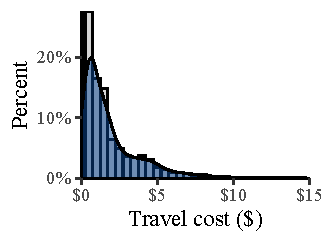
\includegraphics[width=\maxwidth]{figure/plot_costdist-1} 

\end{knitrout}
	  \caption{\centering Travel cost distribution}
	  \label{fig:costdist}
	\end{subfigure}
	\begin{subfigure}[b]{0.325\textwidth}
\begin{knitrout}
\definecolor{shadecolor}{rgb}{0.969, 0.969, 0.969}\color{fgcolor}
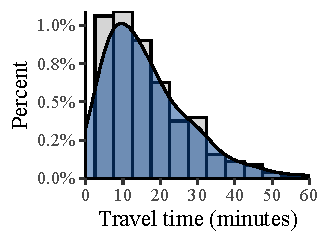
\includegraphics[width=\maxwidth]{figure/plot_timedist-1} 

\end{knitrout}
    \caption{\centering Travel-time distribution}
	  \label{fig:timedist}
  \end{subfigure}
  \begin{subfigure}[b]{0.325\textwidth}
\begin{knitrout}
\definecolor{shadecolor}{rgb}{0.969, 0.969, 0.969}\color{fgcolor}
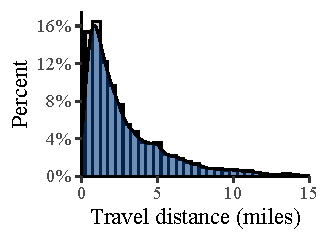
\includegraphics[width=\maxwidth]{figure/plot_distist-1} 

\end{knitrout}
    \caption{\centering Travel distance distribution}
	  \label{fig:distdist}
  \end{subfigure}
  \begin{subfigure}[b]{0.49\textwidth}
\begin{knitrout}
\definecolor{shadecolor}{rgb}{0.969, 0.969, 0.969}\color{fgcolor}
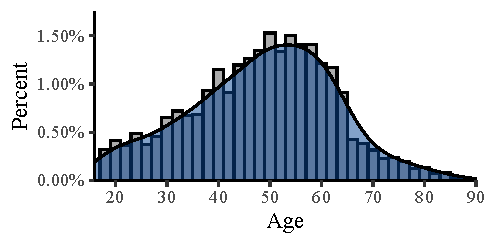
\includegraphics[width=\maxwidth]{figure/plot_agedist-1} 

\end{knitrout}
  \caption{\centering Age distribution}
  \label{fig:agedist}
  \end{subfigure}
    \begin{subfigure}[b]{0.49\textwidth}
\begin{knitrout}
\definecolor{shadecolor}{rgb}{0.969, 0.969, 0.969}\color{fgcolor}
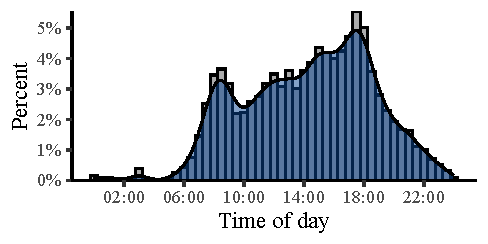
\includegraphics[width=\maxwidth]{figure/plot_toddist-1} 

\end{knitrout}
  \caption{\centering Trip time of day distribution}
  \label{fig:toddist}
  \end{subfigure}
	\caption{Distributions of continuous variables in cleaned Massachusetts Travel Survey dataset}
	\label{fig:contdists}
\end{figure}

It is interesting to note that the age distribution does not match exactly the expected age distribution for the region, particularly with the steep drop at approximately age 65. This is because the data are from a travel survey, meaning that travelers over 65 tend to travel substantially less and may not have been captured, which likely relates to the retirement age. The age distribution was also truncated at 16 years old, which is the minimum age to obtain a driver's license. Another interesting pattern is the large late evening peak in time of day travel, indicating that there is a burst of activity after 5PM. One explanation is that the morning peak is dominated by direct single-destination work trips, while midday and evening trips may be a mixture of trip purposes with multiple trip segments and destinations (e.g., shopping, transporting children, or leisure). 

In order to map how the VOT varies depending on age, income, and trip distance, the variables must be binned into discrete categories. This effectively provides a dissection of the VOT at each bin level, revealing its form that can then be reconstructed through further fitting. The continuous variables were binned in such a way to provide sufficient samples per bin for analysis. Age was binned with equal sized breaks, except at the ends for persons under 20 or over 70 years old. Trip distance was binned using an exponential sequence, and for time of day appropriate breaks were set to match the time of day periods in the travel time skim matrices. The binned continuous variables shown in Table~\ref{tab:data} with their respective frequencies and the median value within each bin for age and distance. This median value will be used later to reconstruct the VOT distributions at the appropriately scaled relative position (e.g., exponential). The median was used instead of the mean in order to minimize the effect of outliers within the binned group. For income, which was already binned in the survey (i.e., no true median was available), a simple midpoint value was used in place of a true calculated median.

%\begin{table}[!h]
%\centering
%%\renewcommand{\arraystretch}{0.8}% Tighter
%\caption{Discrete bins of continuous data from the Massachusetts Travel Survey}
%\label{tab:contdata}
%<<table_binneddata, results="asis", echo=FALSE>>=
%    tables[['data.binned']]
%  @
%\end{table}

\subsubsection{Travel time skims from the Central Transportation Planning Staff's (CTPS) travel demand model}
The travel time skims contain estimated travel times for \numprint{11062} traffic analysis zone (TAZ) pairs in the Greater Boston Area. These travel times are calibrated for the modes of commuter rail, subway (``the T''), local bus, and driving; each estimated for weekday time periods in the morning (AM), midday, evening (PM), and night times (NT). An alternative travel time for each trip in the MTS data was then imputed from the travel time skim matrices based on the trip's corresponding origin-destination pair and time of day.
.

\subsubsection{Monetary travel costs}
The monetary travel costs were compiled from several sources depending on the mode. Public transportation costs were obtained from the Massachusetts Bay Transportation Authority fare structure at the time of the 2011 MTS survey and travel time skims. Within public transportation modes, local bus and subways have a fixed fare, but commuter rail fares were based on a zoned structure, which was imputed based on the traveler's origin and destination. The driving costs were roughly estimated using the average cost per mile of driving, reported by AAA \citep{AAA2018}, and if applicable to the destination, adding the average hourly cost for city street parking (e.g., \$1.25/hour in Boston) and adding tolls if the shortest route traversed one of the five tolled locations (i.e., Massachusetts Turnpike, Sumner Tunnel, Callahan Tunnel, Ted Williams Tunnel, and Tobin Memorial Bridge). Taxi fares were estimated using a typical fare calculation structure which consists of a fixed starting cost, plus a per mile cost and a per hour cost \citep{NUMBEO2019}. All monetary values either originated in 2011 US dollars or were adjusted to 2011 US dollar values using the consumer price index \citep{BLS2019}.


\section{Results}\label{sec:results}
The results of this paper are described as follows. First, estimation results for an overall multinomial logit model using all variables is presented to demonstrate the modeling capability of the data in a conventional discrete choice model. Second, the VOT is estimated for joint pairwise variables to explore VOT variation across multiple variables simultaneously. The purpose of pairwise estimation is to provide a two-dimensional interaction plot to allow for simultaneously studying the relationship between two variables and VOT, which would otherwise be impossible to visualize in higher dimensions. Third, the estimation of VOT across individual variables is presented. While individual variable estimation ignores potentially important variable interactions, the purpose is to help ensure that a more robust result is achieved that is less prone to data sparsity from excess combinatorial variable interactions (e.g., too few samples for a particular variable combination). The individual estimation is then used to create a continuous parameterization for visualization and interpretation purposes.

\subsection{Full multinomial model results}
Before investigating VOT variation, a full multinomial discrete choice model is estimated using all of the available variables in a combined model. The purpose of this is to help validate the viability of the travel survey data and to simply demonstrate its modeling capability. The estimation results for the full multinomial model are shown in Table~\ref{tab:fullmod}, with the ``drive'' alternative being omitted as the reference category of the model. Overall the model achieved a McFadden $R^2$ of 0.84, which suggests reasonably good fit results, but several variables and intercepts yielded less than ideal results with unexpected positive coefficients and/or insignificance. This may be attributed to noisy data and model complexity, potentially resulting in over-fitting. A simpler or more refined model, as well as additional data cleaning could improve the model. However, for the purpose of investigating VOT variation, the results are satisfactory.

\begin{table}[!h]
%	\renewcommand{\arraystretch}{0.7}% Tighter
	\centering
	\setlength{\tabcolsep}{2pt}
	\caption{Multinomial model results}
	\label{tab:fullmod}
\begingroup\fontsize{8}{10}\selectfont

\begin{tabular}{lllllllllllll}
\toprule
\multicolumn{1}{c}{\textbf{ }} & \multicolumn{3}{c}{\textbf{Taxi}} & \multicolumn{3}{c}{\textbf{Bus}} & \multicolumn{3}{c}{\textbf{Subway}} & \multicolumn{3}{c}{\textbf{Rail}} \\
\cmidrule(l{3pt}r{3pt}){2-4} \cmidrule(l{3pt}r{3pt}){5-7} \cmidrule(l{3pt}r{3pt}){8-10} \cmidrule(l{3pt}r{3pt}){11-13}
Variable & $\beta$ & SE & p-value & $\beta$ & SE & p-value & $\beta$ & SE & p-value & $\beta$ & SE & p-value\\
\midrule
Intercept & -1.33 & 0.88 & 1.3e-01 & -4.35 & 1.13 & 1.1e-04 *** & 13.03 & 2340.50 & 1.0e+00 & 5.86 & 0.81 & 5.2e-13 ***\\
Age & -0.01 & 0.01 & 6.2e-01 & -0.03 & 0.00 & $<$ 2.2e-16 *** & -0.03 & 0.00 & $<$ 2.2e-16 *** & -0.02 & 0.01 & 4.2e-03 **\\
Cost & -0.58 & 0.05 & $<$ 2.2e-16 *** & 6.21 & 0.75 & 2.2e-16 *** & -4.58 & 1170.25 & 1.0e+00 & 0.30 & 0.08 & 1.3e-04 ***\\
Gender & -0.17 & 0.33 & 6.1e-01 & -0.04 & 0.09 & 6.6e-01 & 0.17 & 0.10 & 7.9e-02 & -0.21 & 0.18 & 2.5e-01\\
Income - 25,000-49,999 & -2.14 & 0.59 & 2.7e-04 *** & -2.46 & 0.15 & $<$ 2.2e-16 *** & -0.78 & 0.19 & 4.4e-05 *** & -2.23 & 0.36 & 4.9e-10 ***\\
Income - 50,000-74,999 & -2.13 & 0.53 & 6.1e-05 *** & -2.82 & 0.15 & $<$ 2.2e-16 *** & -0.74 & 0.19 & 7.1e-05 *** & -1.93 & 0.34 & 1.1e-08 ***\\
Income - 75,000-99,999 & -3.46 & 0.74 & 2.8e-06 *** & -3.41 & 0.17 & $<$ 2.2e-16 *** & -0.85 & 0.19 & 7.9e-06 *** & -1.85 & 0.33 & 3.3e-08 ***\\
Income - 100,000-149,999 & -2.53 & 0.53 & 1.7e-06 *** & -3.81 & 0.16 & $<$ 2.2e-16 *** & -1.39 & 0.18 & 2.6e-14 *** & -2.33 & 0.30 & 1.3e-14 ***\\
Income - $\geq$ 150,000 & -1.98 & 0.44 & 7.5e-06 *** & -3.96 & 0.17 & $<$ 2.2e-16 *** & -1.55 & 0.18 & $<$ 2.2e-16 *** & -2.28 & 0.30 & 4.2e-14 ***\\
Trip duration & 0.65 & 0.05 & $<$ 2.2e-16 *** & -0.16 & 0.00 & $<$ 2.2e-16 *** & -0.17 & 0.00 & $<$ 2.2e-16 *** & -0.25 & 0.01 & $<$ 2.2e-16 ***\\
Trip purpose - Recreation & -0.19 & 0.63 & 7.7e-01 & 2.14 & 0.25 & $<$ 2.2e-16 *** & 2.14 & 0.32 & 2.8e-11 *** & 1.93 & 0.71 & 6.7e-03 **\\
Trip purpose - Shopping/errands & 0.13 & 0.57 & 8.2e-01 & 2.05 & 0.23 & $<$ 2.2e-16 *** & 1.74 & 0.32 & 4.5e-08 *** & 1.73 & 0.69 & 1.3e-02 *\\
Trip purpose - Work/school & 0.76 & 0.56 & 1.7e-01 & 3.92 & 0.23 & $<$ 2.2e-16 *** & 3.72 & 0.30 & $<$ 2.2e-16 *** & 3.76 & 0.66 & 1.5e-08 ***\\
Time of day - Midday & 0.03 & 0.50 & 9.6e-01 & -1.11 & 0.13 & $<$ 2.2e-16 *** & -0.88 & 0.15 & 1.1e-08 *** & -1.28 & 0.28 & 4.6e-06 ***\\
Time of day - Night & 1.27 & 0.53 & 1.6e-02 * & 0.57 & 0.20 & 3.9e-03 ** & -0.63 & 0.17 & 2.4e-04 *** & -0.22 & 0.31 & 4.8e-01\\
Time of day - PM & -1.92 & 0.70 & 6.2e-03 ** & -0.63 & 0.14 & 3.7e-06 *** & -0.54 & 0.14 & 1.5e-04 *** & 0.04 & 0.25 & 8.7e-01\\
\bottomrule
\multicolumn{13}{l}{McFadden $R^2=0.75$}\\
\multicolumn{13}{l}{\textsuperscript{*} Significance level codes: '***' 99.99\%, '**' 99\%, '*' 95\%}\\
\end{tabular}
\endgroup{}


\end{table}

\pagebreak

\subsection{Pairwise variable joint VOT estimation results}
The pairwise variables (i.e., two interaction variables using Equation~\eqref{eq:twointeract}) were estimated as discrete variables for all unique variable pair combinations. Regression estimates for the joint pairwise interaction models are not displayed in their entirety because there is a combined total of 349 coefficients, which are too many to display in this paper, full results can be found on the public GitHub repository \url{https://github.com/nick-fournier/Value-of-Time-Exploration}. The resulting joint VOTs are shown in Figure~\ref{fig:jointplots}, with errors summarized in Table~\ref{tab:jterror}. The joint models achieved $R^2$ values between 0.53 and 0.58, with the majority of variables being statistically significant. However, the resulting VOTs also possessed an extremely large range of error in each case, calculated using Equation~\eqref{eq:error}.

\begin{table}[!h]
	\centering
	\setlength{\tabcolsep}{4pt}
	%\renewcommand{\arraystretch}{0.7}% Tighter
	\caption{Summary statistics for joint VOT error}
	\label{tab:jterror}
\begingroup\fontsize{8}{10}\selectfont

\begin{tabular}{lr>{\raggedleft\arraybackslash}p{0.5in}rr>{\raggedleft\arraybackslash}p{0.5in}r>{\raggedleft\arraybackslash}p{0.5in}>{\raggedright\arraybackslash}p{0.5in}}
\toprule
\multicolumn{1}{c}{ } & \multicolumn{6}{c}{Value of time error} \\
\cmidrule(l{3pt}r{3pt}){2-7}
Model & Minimum & First Quantile & Median & Mean & Third Quantile & Maximum & McFadden $R^2$ & Significant variables\\
\midrule
Age$\times$Trip purpose & 4.98 & 17.59 & 25.03 & 132.78 & 41.07 & 1395.32 & 0.56 & 55 of 60\\
Age$\times$Time of day & 4.24 & 13.78 & 26.41 & 72.43 & 52.73 & 615.02 & 0.55 & 55 of 60\\
Distance$\times$Age & 1.96 & 19.95 & 36.22 & 275.93 & 412.00 & 2463.84 & 0.57 & 76 of 102\\
Distance$\times$Trip purpose & 2.45 & 15.76 & 25.84 & 307.83 & 515.06 & 2582.28 & 0.58 & 52 of 60\\
Distance$\times$Time of day & 5.76 & 11.81 & 40.62 & 1550.21 & 193.05 & 36577.78 & 0.56 & 51 of 60\\
Gender$\times$Age & 7.41 & 16.53 & 19.00 & 34.70 & 22.56 & 238.32 & 0.54 & 31 of 32\\
Gender$\times$Income & 7.15 & 11.40 & 15.23 & 16.64 & 19.48 & 32.61 & 0.55 & 28 of 28\\
Gender$\times$Distance & 7.19 & 9.33 & 16.08 & 130.11 & 90.80 & 998.04 & 0.55 & 30 of 32\\
Gender$\times$Trip purpose & 9.99 & 12.15 & 17.90 & 17.95 & 23.79 & 26.53 & 0.55 & 20 of 20\\
Gender$\times$Time of day & 4.00 & 11.70 & 15.98 & 22.33 & 26.36 & 65.54 & 0.53 & 20 of 20\\
Income$\times$Age & 7.19 & 15.96 & 26.47 & 93.19 & 41.43 & 710.53 & 0.56 & 80 of 88\\
Income$\times$Distance & 7.87 & 17.91 & 35.77 & 622.37 & 190.09 & 19865.73 & 0.58 & 75 of 88\\
Income$\times$Trip Purpose & 3.48 & 15.42 & 24.34 & 30.63 & 40.98 & 76.47 & 0.58 & 52 of 52\\
Income$\times$Time of day & 3.81 & 13.04 & 17.74 & 65.33 & 39.46 & 927.82 & 0.56 & 51 of 52\\
Trip purpose$\times$Time of day & 4.56 & 11.26 & 22.08 & 36.25 & 49.09 & 184.68 & 0.56 & 36 of 36\\
\bottomrule
\end{tabular}
\endgroup{}


\end{table}

\begin{figure}[H]
	\centering
	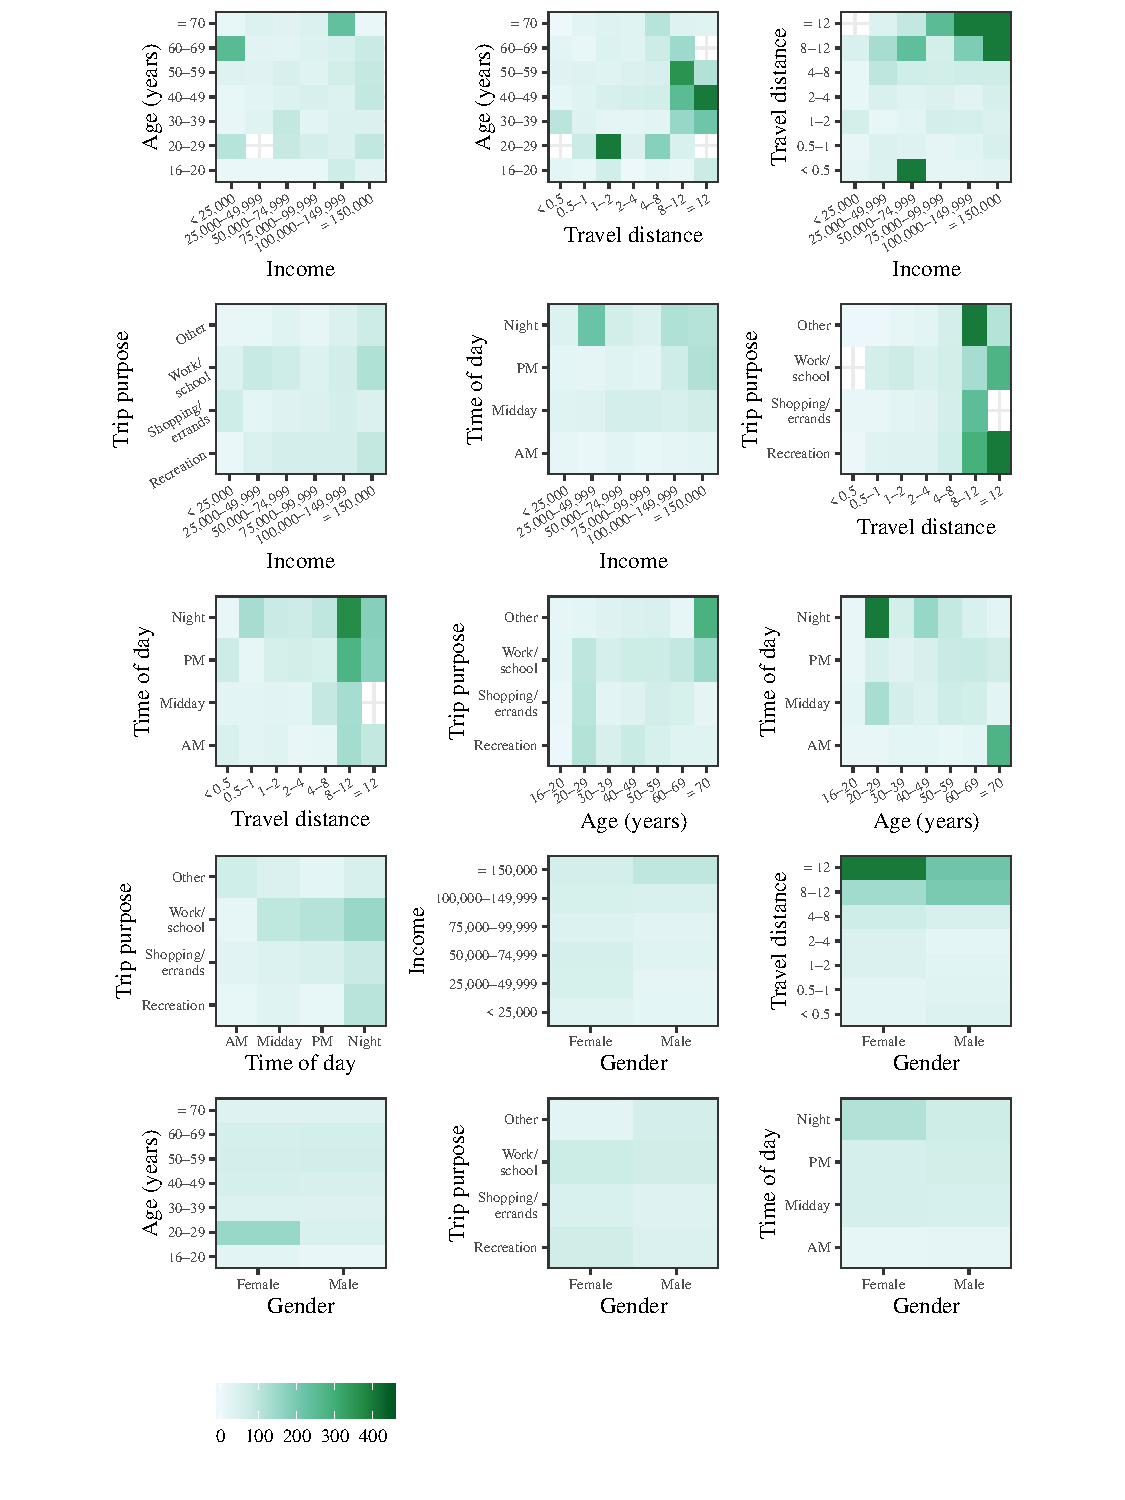
\includegraphics[width=\textwidth]{localdata/jointplot}
	\caption{Joint variable VOT plots}
	\label{fig:jointplots}
\end{figure}

\subsection{Individual variable value of time estimation results}
The results of the individually estimated study variable models (i.e., one interaction variable) are summarized in Table~\ref{tab:regresults}. In general all models achieved fairly good fit results, yielding McFadden $R^2$ values between 0.53 and 0.65.

\begin{table}[H]
\centering
\caption{Summary of individual variable model estimation results}
\label{tab:regresults}
\begingroup\fontsize{8}{10}\selectfont

\begin{tabular}{lrllllllll}
\toprule
\multicolumn{2}{c}{ } & \multicolumn{4}{c}{Travel time} & \multicolumn{4}{c}{Travel cost} \\
\cmidrule(l{3pt}r{3pt}){3-6} \cmidrule(l{3pt}r{3pt}){7-10}
Variable & VOT & $\beta$ & SE & z-value & p-value & $\beta$ & SE & z-value & p-value\\
\midrule
\addlinespace[0.3em]
\multicolumn{10}{l}{\textbf{Age model, $McFadden~R^2 = 0.54$}}\\
\hline
\hspace{1em}16-20 & 14.2 & -0.09 & 5.58e-03 & -16.66 & $<$ 2.2e-16 *** & -0.39 & 8.62e-02 & -4.55 & 5.5e-06 ***\\
\hspace{1em}20-29 & 82.8 & -0.10 & 3.48e-03 & -28.98 & $<$ 2.2e-16 *** & -0.07 & 1.93e-02 & -3.80 & 1.5e-04 ***\\
\hspace{1em}30-39 & 39.1 & -0.15 & 4.10e-03 & -35.97 & $<$ 2.2e-16 *** & -0.23 & 2.49e-02 & -9.09 & $<$ 2.2e-16 ***\\
\hspace{1em}40-49 & 50.9 & -0.16 & 3.70e-03 & -43.49 & $<$ 2.2e-16 *** & -0.19 & 1.80e-02 & -10.54 & $<$ 2.2e-16 ***\\
\hspace{1em}50-59 & 58.6 & -0.16 & 3.29e-03 & -47.33 & $<$ 2.2e-16 *** & -0.16 & 1.43e-02 & -11.16 & $<$ 2.2e-16 ***\\
\hspace{1em}60-69 & 56.0 & -0.15 & 3.96e-03 & -38.51 & $<$ 2.2e-16 *** & -0.16 & 1.85e-02 & -8.82 & $<$ 2.2e-16 ***\\
\hspace{1em}$\geq$ 70 & 35.4 & -0.17 & 7.00e-03 & -24.17 & $<$ 2.2e-16 *** & -0.29 & 4.27e-02 & -6.71 & 1.9e-11 ***\\
\addlinespace[0.3em]
\multicolumn{10}{l}{\textbf{Gender, $McFadden~R^2 = 0.53$}}\\
\hline
\hspace{1em}Female & 50.4 & -0.14 & 2.45e-03 & -58.68 & $<$ 2.2e-16 *** & -0.17 & 1.20e-02 & -14.34 & $<$ 2.2e-16 ***\\
\hspace{1em}Male & 48.1 & -0.15 & 2.66e-03 & -54.65 & $<$ 2.2e-16 *** & -0.18 & 1.26e-02 & -14.39 & $<$ 2.2e-16 ***\\
\addlinespace[0.3em]
\multicolumn{10}{l}{\textbf{Income model, $McFadden~R^2 = 0.55$}}\\
\hline
\hspace{1em}< 25,000 & 26.9 & -0.09 & 2.62e-03 & -35.56 & $<$ 2.2e-16 *** & -0.21 & 3.15e-02 & -6.59 & 4.5e-11 ***\\
\hspace{1em}25,000-49,999 & 33.2 & -0.14 & 4.14e-03 & -34.37 & $<$ 2.2e-16 *** & -0.26 & 3.21e-02 & -7.99 & 1.3e-15 ***\\
\hspace{1em}50,000-74,999 & 42.2 & -0.15 & 4.11e-03 & -37.19 & $<$ 2.2e-16 *** & -0.22 & 2.52e-02 & -8.61 & $<$ 2.2e-16 ***\\
\hspace{1em}75,000-99,999 & 32.3 & -0.16 & 4.46e-03 & -36.36 & $<$ 2.2e-16 *** & -0.30 & 2.90e-02 & -10.38 & $<$ 2.2e-16 ***\\
\hspace{1em}100,000-149,999 & 50.1 & -0.18 & 4.48e-03 & -39.41 & $<$ 2.2e-16 *** & -0.21 & 1.86e-02 & -11.36 & $<$ 2.2e-16 ***\\
\hspace{1em}$\geq$ 150,000 & 71.7 & -0.18 & 4.14e-03 & -42.63 & $<$ 2.2e-16 *** & -0.15 & 1.27e-02 & -11.64 & $<$ 2.2e-16 ***\\
\addlinespace[0.3em]
\multicolumn{10}{l}{\textbf{Mode model, $McFadden~R^2 = 0.65$}}\\
\hline
\hspace{1em}Rail & 10.4 & -0.18 & 6.48e-03 & -28.51 & $<$ 2.2e-16 *** & -1.07 & 6.66e-02 & -16.04 & $<$ 2.2e-16 ***\\
\hspace{1em}Drive & 4.0 & 0.05 & 5.30e-03 & 8.85 & $<$ 2.2e-16 *** & 0.71 & 1.98e-02 & 35.73 & $<$ 2.2e-16 ***\\
\hspace{1em}Bus & 5.9 & -0.16 & 3.68e-03 & -42.25 & $<$ 2.2e-16 *** & -1.57 & 5.55e-02 & -28.27 & $<$ 2.2e-16 ***\\
\hspace{1em}Subway & 6.6 & -0.17 & 3.96e-03 & -43.66 & $<$ 2.2e-16 *** & -1.57 & 5.01e-02 & -31.28 & $<$ 2.2e-16 ***\\
\hspace{1em}Taxi & 52.2 & 0.99 & 3.93e-02 & 25.13 & $<$ 2.2e-16 *** & 1.14 & 3.78e-02 & 30.03 & $<$ 2.2e-16 ***\\
\addlinespace[0.3em]
\multicolumn{10}{l}{\textbf{Travel distance model, $McFadden~R^2 = 0.55$}}\\
\hline
\hspace{1em}< 0.5 & 28.0 & -0.25 & 1.05e-02 & -23.54 & $<$ 2.2e-16 *** & -0.53 & 6.24e-02 & -8.45 & $<$ 2.2e-16 ***\\
\hspace{1em}0.5-1 & 25.5 & -0.19 & 5.59e-03 & -34.71 & $<$ 2.2e-16 *** & -0.46 & 4.39e-02 & -10.43 & $<$ 2.2e-16 ***\\
\hspace{1em}1-2 & 34.1 & -0.16 & 3.44e-03 & -46.37 & $<$ 2.2e-16 *** & -0.28 & 2.79e-02 & -10.08 & $<$ 2.2e-16 ***\\
\hspace{1em}2-4 & 32.6 & -0.13 & 2.75e-03 & -47.50 & $<$ 2.2e-16 *** & -0.24 & 2.50e-02 & -9.61 & $<$ 2.2e-16 ***\\
\hspace{1em}4-8 & 57.1 & -0.13 & 3.47e-03 & -38.36 & $<$ 2.2e-16 *** & -0.14 & 1.38e-02 & -10.16 & $<$ 2.2e-16 ***\\
\hspace{1em}8-12 & 157.8 & -0.11 & 5.22e-03 & -21.42 & $<$ 2.2e-16 *** & -0.04 & 9.95e-03 & -4.27 & 2.0e-05 ***\\
\hspace{1em}$\geq$ 12 & 291.3 & -0.10 & 8.36e-03 & -11.54 & $<$ 2.2e-16 *** & -0.02 & 1.11e-02 & -1.80 & 7.2e-02\\
\addlinespace[0.3em]
\multicolumn{10}{l}{\textbf{Trip purpose model, $McFadden~R^2 = 0.55$}}\\
\hline
\hspace{1em}Other & 41.5 & -0.28 & 1.03e-02 & -26.72 & $<$ 2.2e-16 *** & -0.40 & 4.08e-02 & -9.79 & $<$ 2.2e-16 ***\\
\hspace{1em}Recreation & 54.6 & -0.16 & 4.30e-03 & -37.08 & $<$ 2.2e-16 *** & -0.17 & 1.97e-02 & -8.86 & $<$ 2.2e-16 ***\\
\hspace{1em}Shopping/errands & 42.2 & -0.16 & 3.35e-03 & -48.09 & $<$ 2.2e-16 *** & -0.23 & 1.93e-02 & -11.83 & $<$ 2.2e-16 ***\\
\hspace{1em}Work/school & 70.2 & -0.12 & 2.27e-03 & -54.59 & $<$ 2.2e-16 *** & -0.11 & 9.86e-03 & -10.73 & $<$ 2.2e-16 ***\\
\addlinespace[0.3em]
\multicolumn{10}{l}{\textbf{Time-of-day model, $McFadden~R^2 = 0.53$}}\\
\hline
\hspace{1em}AM & 17.2 & -0.14 & 3.79e-03 & -36.60 & $<$ 2.2e-16 *** & -0.48 & 3.27e-02 & -14.79 & $<$ 2.2e-16 ***\\
\hspace{1em}Midday & 53.3 & -0.15 & 2.88e-03 & -53.32 & $<$ 2.2e-16 *** & -0.17 & 1.41e-02 & -12.26 & $<$ 2.2e-16 ***\\
\hspace{1em}PM & 57.5 & -0.15 & 3.22e-03 & -45.51 & $<$ 2.2e-16 *** & -0.15 & 1.56e-02 & -9.83 & $<$ 2.2e-16 ***\\
\hspace{1em}Night & 91.8 & -0.12 & 3.24e-03 & -37.99 & $<$ 2.2e-16 *** & -0.08 & 1.24e-02 & -6.52 & 7.2e-11 ***\\
\bottomrule
\multicolumn{10}{l}{\textsuperscript{*} Significance level codes: '***' 99.99\%, '**' 99\%, '*' 95\%}\\
\end{tabular}
\endgroup{}


\end{table}

In all models, all input variables achieved >99\% significance and almost all models yielded negative coefficients. The exception being for taxi and drive modes, where a positive coefficient was associated with travel cost and time. This result may be due to different trip purposes (e.g., leisure versus commute travel) or unaccounted taste preferences, such as taxis that are slower than driving (e.g., wait time), but offer a premium service at a higher costs. More refined modeling approaches are necessary to resolve this.

\subsubsection{Individual categorical variable exploration results}

The categorical variable results for mode, purpose, and time of day, and gender are summarized in Figure~\ref{fig:votcats}, yielding somewhat surprising results. Commuter rail, work/school trips, and night time trips yielded the highest VOT among modes, trip purpose, and time of day, respectively. However, the highest VOT was also associated with the highest range of error in each case while the majority of other points had a relatively small range of error. 

\begin{figure}[!h]
  \centering
  \begin{subfigure}[t]{0.3\textwidth}
\begin{knitrout}
\definecolor{shadecolor}{rgb}{0.969, 0.969, 0.969}\color{fgcolor}
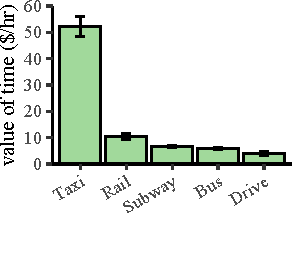
\includegraphics[width=\maxwidth]{figure/plot_votmode-1} 

\end{knitrout}
	  \caption{\centering Travel mode}
	  \label{fig:votmode}
	\end{subfigure}
	\begin{subfigure}[t]{0.26\textwidth}
\begin{knitrout}
\definecolor{shadecolor}{rgb}{0.969, 0.969, 0.969}\color{fgcolor}
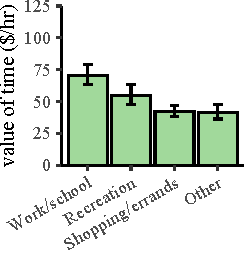
\includegraphics[width=\maxwidth]{figure/plot_votpurpose-1} 

\end{knitrout}
    \caption{\centering Trip purpose}
	  \label{fig:votpurpose}
  \end{subfigure}
  \begin{subfigure}[t]{0.26\textwidth}
\begin{knitrout}
\definecolor{shadecolor}{rgb}{0.969, 0.969, 0.969}\color{fgcolor}
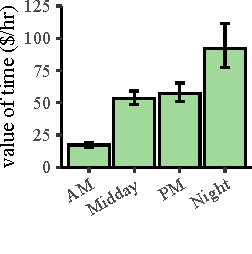
\includegraphics[width=\maxwidth]{figure/plot_vottod-1} 

\end{knitrout}
    \caption{\centering Time of day}
	  \label{fig:vottod}
  \end{subfigure}
  \begin{subfigure}[t]{0.15\textwidth}
\begin{knitrout}
\definecolor{shadecolor}{rgb}{0.969, 0.969, 0.969}\color{fgcolor}
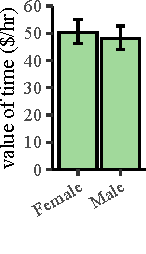
\includegraphics[width=\maxwidth]{figure/plot_votgend-1} 

\end{knitrout}
	\caption{\centering Gender}
	\label{fig:votgend}
	\end{subfigure}
	\caption{VOT for categorical variables}
	\label{fig:votcats}
\end{figure}

\subsubsection{Individual continuous variable exploration results}

The binned continuous variables are plotted in Figure~\ref{fig:fits}. For demonstration purposes, the data points are fitted with a parametric model, fitted to each continuous variable. The fitting results are summarized in Table~\ref{tab:parafit}. Income and travel distance both yielded a recognizable exponential form, which were easily fitted as log-linear models with an $R^2$ of 0.74 and 0.98, respectively. Age resulted in an arc shaped pattern that was fitted to a Gaussian function, yielding an $R^2$ of 0.999. 

\begin{figure}[H]
  \centering
  \begin{subfigure}[b]{0.32\textwidth}
\begin{knitrout}
\definecolor{shadecolor}{rgb}{0.969, 0.969, 0.969}\color{fgcolor}
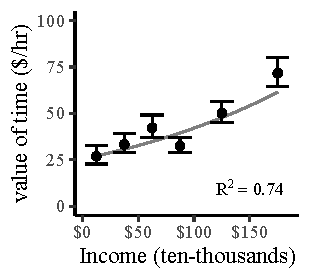
\includegraphics[width=\maxwidth]{figure/plot_incfit-1} 

\end{knitrout}
	  \caption{\centering Fitted VOT as a log-linear function of income}
	  \label{fig:incfit}
	\end{subfigure}
	\begin{subfigure}[b]{0.32\textwidth}
\begin{knitrout}
\definecolor{shadecolor}{rgb}{0.969, 0.969, 0.969}\color{fgcolor}
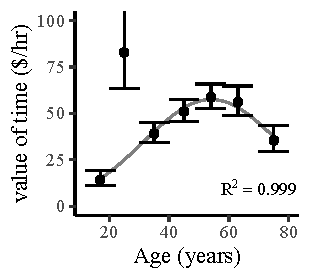
\includegraphics[width=\maxwidth]{figure/plot_agefit-1} 

\end{knitrout}
    \caption{\centering Fitted VOT as a Gaussian function of age}
	  \label{fig:agefit}
  \end{subfigure}
  \begin{subfigure}[b]{0.32\textwidth}
\begin{knitrout}
\definecolor{shadecolor}{rgb}{0.969, 0.969, 0.969}\color{fgcolor}
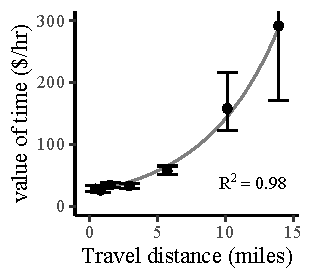
\includegraphics[width=\maxwidth]{figure/plot_distfit-1} 

\end{knitrout}
    \caption{\centering Fitted VOT as a log-linear function of travel distance}
	  \label{fig:distfit}
  \end{subfigure}
	\caption{Fitted VOT distribution for continuous variables}
	\label{fig:fits}
\end{figure}

The parameters in Table~\ref{tab:parafit} present the intercept $\alpha$ and the exponential rate coefficient $\beta$ for the log-linear models for income and travel distance. The Gaussian model for age has parameters for the mean $\mu$, standard deviation $\sigma$, and a scaling parameter $b$. In order to produce a coefficient at a reasonable scale (i.e., not extremely small), income was also adjusted on a fixed unit scale of \$10,000 for $x$, while age and travel distance were left in units of miles and years.

\begin{table}[!h]
\centering
\caption{Summary of parametric fitting results}
\label{tab:parafit}
\begingroup\fontsize{9}{11}\selectfont

\begin{tabular}{lllllllll}
\toprule
\multicolumn{3}{c}{Model} & \multicolumn{5}{c}{Parameters} \\
\cmidrule(l{3pt}r{3pt}){1-3} \cmidrule(l{3pt}r{3pt}){4-8}
Variable & Unit & Function & $\alpha$ & $\beta$ & $b$ & $\mu$ & $\sigma$ & $R^2$\\
\midrule
Income & \$10,000 & $VOT(x)=e^{\alpha+\beta x}$ & 3.232 & 0.051 &  &  &  & 0.741\\
Travel distance & Miles & $VOT(x)=e^{\alpha+\beta x}$ & 3.124 & 0.183 &  &  &  & 0.984\\
Age & Years & $VOT(x)=\frac{b}{\sigma\sqrt{2\pi}}e^{-\frac{(x-\mu)^2}{2\sigma^2}}$ &  &  & 3235.246 & 54.077 & 22.466 & 0.999\\
\bottomrule
\end{tabular}
\endgroup{}


\end{table}

\section{Discussion}\label{sec:discussion}
This study utilized a household travel survey to construct a revealed preference dataset with imputed alternatives to estimate multinomial discrete choice models for mode choice in order to measure the VOT across several study variables. The objective is to investigate whether any patterns or relationships exist between the VOT and common demographic and travel variables (e.g., age, income, gender, purpose, time of day, and trip distance). The purpose is to reveal these underlying patterns in the VOT, helping to provide a better understanding of their shape for use in future research and practice. A better understanding of the VOT is important to the development of more informed and refined transportation models, but also helps focus research by exposing questions that require further investigation on why such relationships exist. The following subsections discuss the findings for VOT by each of the study variable types. 

\subsection{Age, income, and travel distance}
The VOT by age was found to follow a Gaussian function (a normal curve), with the crest (the mean) at approximately 54 years old, suggesting that for some reason older travelers tend to have a lower VOT and middle age the highest. There are many possible explanations for this result. Perhaps it has to do with the stage of life people are in (e.g., fewer time constraints when older and younger, or higher income and responsibilities at middle age). Though less plausible, it could also simply be a generational phenomenon. Further research is necessary to explain this, either through explanatory variables or through longitudinal studies over time. Regardless, if age does possess a Gaussian or general ``U-shaped'' VOT function, this will have very critical modeling implications. Any model estimating age linearly, or log-linearly, will fail to accurately capture this curve and merely find some average point with severe error.

Although the Gaussian function was overall a good fit for VOT by age with an $R^2$ of  0.999, there was one outlier for ages 20-29, shown in Table~\ref{tab:regresults} and Figure~\ref{fig:agefit}. The issue can be isolated to travel cost because unlike the travel time coefficient, the cost coefficient appears to be very low and relatively out of step with the other cost coefficients. This causes an imbalance in the VOT calculation of $VOT = \frac{\beta_{time}}{\beta_{cost}}$, causing VOT to dramatically increase if estimation error is not systematic across both time and cost. One possible explanation is that 20-29 year olds often have subsidized travel, such as student transit passes or a car owned by their parents, thus having an overvalued travel cost in the data. This problem is potentially magnified by the huge number of colleges and universities in Massachusetts. These externalities are difficult to explain with the given data set, but future surveys and modeling approaches could better account for such transfers of costs in more detail. 

The results also show that the VOT varies log-linearly with both income and travel distance. However, the log-linear coefficient (exponential rate of increase) for income of only 5.1e-06 implies a much more gradual upward curve compared to travel distance, which has a coefficient of 0.18. This means that travel distance (and total travel time) tends to dominate the overall VOT as trip length increases. The importance of this is that not accounting for travel distance in a transportation model has very serious modeling implications. For example, a ten mile trip has a VOT approximately 5.2 times higher than a one mile trip.

Travel distance is also a spatial variable, which can vary by location of work, home, and choice of leisure or other personal activities. Furthermore, there is likely to be areas of correlation or ``self selection'' bias among variables. For example, particularly high/low income people or industries may be concentrated in specific areas. Higher income travelers may choose to live closer to employment at a premium, or in contrast could choose to live in wealthy remote suburb with direct commuter rail access. In either case, this could confound any model estimation. Further spatial analysis is necessary to determine the effect that this has on VOT estimation in regards to travel distance.

Travel distance is also a spatial variable, which can vary by location of work, home, and choice of leisure or other personal activities. Furthermore, there is likely to be areas of correlation or ``self selection'' bias among variables. For example, particularly high/low income people or industries may be concentrated in specific areas. Higher income travelers may choose to live closer to employment at a premium, or in contrast could choose to live in wealthy remote suburb with direct commuter rail access. In either case, this could confound any model estimation. Further spatial analysis is necessary to determine the effect that this has on VOT estimation in regards to travel distance.

\subsection{Mode, trip purpose, time of day, and gender}
The categorical variables showed that commuter rail, work/school trips, and night time travel have the highest VOTs. The result for mode is somewhat interesting considering that the VOT for commuter rail, a public transportation mode, was much higher than the other public transportation modes of subway and bus. It perhaps has more to do with intersectionality of users, for example that commuter rail riders are primarily higher-income travelers using it for work trips, both of which have a very high VOT. However, the highest VOT in mode, trip purpose, and time of day, also showed the greatest range of error, suggesting the result may be inaccurate due to unexplained variation (e.g., type of people making work/school trips) or small sample sizes (e.g., night time travel).

Moreover, despite the detailed and systematic assignment of imputed travels costs for the mode alternatives, there are likely to be many unaccounted cost factors, such as availability of street parking, availability of automobiles, trip encumbrances (e.g., transporting goods, groceries, children, disabilities, etc.), discounted toll/fare passes, etc. There is likely an unimaginable variety of factors affecting travel cost and behavior. 


Another serious issue are the positive coefficients associated with driving and taxi modes. The exact reasoning for this is difficult to determine and may be affected by the small sample size of only \numprint{72} taxi trips. One possible explanation is that taxis are unique in that they can have longer travel times than driving, but cost much more due to the added convenience they offer to travelers. This convenience is not captured in the simple models used in this paper, resulting in a negative value when compared to automobiles. However, this does not entirely explain the positive coefficient for driving. More sophisticated models are necessary to account for this, such as accounting for when no automobile is available at the trip level, not just at the personal or household level. Moreover, transit modes other than the commuter rail in Boston are not distance based, meaning that the monetary cost function is generally flat or stepped over time and distance, introducing further modeling challenges.

Overall, gender had little difference in the VOT. However, when interacting with variables several interesting insights emerge. It would appear that younger women, women taking longer distance trips over 12 miles, and women taking night time trips have a much higher VOT compared to men. The reason for these differences is difficult to speculate, but some possible hypotheses could be additional family responsibilities when commuting or fear/risk of assault during night trips. For example, young men may feel comfortable walking to taking public transit at night while young women may not and are forced to choose a more expensive travel mode or time of day.

\section{Conclusions}\label{sec:conclusion}

This study estimated the VOT across discrete dissections of important modeling variables to explore its variation. The variables are both categorical, such as mode, trip purpose, time of day, and gender; but also continuous variables of income, age, and travel distance. The purpose is to provide a broader understanding of how the VOT varies and determine possible functional form that could be obscured by direct model estimation, particularly across the continuous variables. Although this study utilized fairly crude methods to dissect and visualize the VOT, the results provide valuable insights. In particular, the VOT has a Gaussian form across age, and a steeply increasing exponential shape across travel distance and income. Furthermore, there are also valuable findings in the VOT varying across gender and time of day that yield important considerations for future transportation models when making assumptions about when and how people travel.

These findings are important to both transport models that utilize a VOT, but also in helping guide future research on understanding and modeling the VOT. There is further work to be done to address the limitations and unresolved questions in this study, such as a more precise accounting for travel costs (e.g., parking and tolls), further investigation into the Gaussian form of VOT over age, and a spatial analysis for the VOT and associated factors. Moreover, there is a lack of understanding on how VOT varies across sensitive demographic and socio-economic variables, such as race and ethnicity and other sensitive factors often overlooked in travel models. To investigate these issues further, a mixed logit would be a logical next step. However, a mixed logit model requires a parametric function to be known a priori for the continuous ``mixing'' variable. Findings from this current study could serve as a useful step towards a more sophisticated mixed-logit model estimation and analysis.

This analysis approach could also be applied to other household surveys, such as the National Household Travel Survey (NHTS) \citep{NHTS2017}. Unfortunately, while the NHTS is a much larger survey spanning the entire United States, it does not contain all trip costs, only annual fuel cost for driving. For the MTS data, these costs were able to be meticulously imputed using local transit fare structures for each transit mode and trip. Performing this task for the entire NHTS data set would be an enormous task given the many different transit systems in the United States. However, with sufficient resources to perform this task, or if future NHTS collects transit costs, expanding this work using NHTS data would help provide important VOT results for broader policy implications beyond just Massachusetts.


%TC:ignore
\section{Author contributions}
The authors confirm contribution to the paper as follows: study conception, data collection, analysis, and manuscript drafting by Nicholas Fournier. Eleni Christofa provided critical feedback, research supervision, and manuscript editing.

\section{Acknowledgments}
This research was funded in part by the US DOE's Advanced Research Projects Agency-Energy (ARPA-E) under the Traveler Response Architecture using Novel Signaling for Network Efficiency in Transportation (TRANSNET) program, with Award Number DE-AR0000611.

%\newpage

\bibliographystyle{trb}
\bibliography{trb_vot}

\pagebreak

%\section{Appendix}
%\begin{center}
%	\renewcommand{\arraystretch}{0.8}% Tighter
%	\centering
% <<table_appendix, results="asis", echo=FALSE>>=
%   tables[['jtregresults']]
%   @
%\end{center}
%TC:endignore 
\end{document}
